% 8Queens.tex
\documentclass[12pt,letterpaper]{letter}
\usepackage{fullpage,color,graphicx}
\usepackage[procnames]{listings}
\pagenumbering{gobble}

\newcommand{\assignment}{8 Queens}
\newcommand{\myinfo}
{Darin Critchlow
\\CSIS 2430-001}
\newcommand{\assignmentDescription}
{The eight queens puzzle is the problem of placing eight chess queens on an $8\times8$ chessboard so that no two queens attack each other. Thus, a solution requires that no two queens share the same row, column, or diagonal. The eight queens puzzle is an example of the more general n-queens problem of placing \emph{n} queens on an $n\times n$ chessboard, where solutions exist for all natural numbers n with the exception of $n=2$ and $n=3$.
}
\newcommand{\worked}
{
Everything worked properly
}
\newcommand{\didntwork}
{
Everything worked properly
}
\newcommand{\comments}
{
It was more difficult than I first thought it would be to decide on what data structure to use to store the solutions. I wanted a way to keep the row and column so that I could output a ‘pretty’ version to the console. I decided to use a set structure because it provided very convenient methods to iterate through row and column values.
}

\begin{document}

\LARGE\textbf{\assignment{}}

\normalsize\myinfo{}

\textbf{\underline{Objective:}}

\textbf{\assignmentDescription{}}

\textbf{\underline{What Worked:}}

\worked{}

\textbf{\underline{What Didn't Work:}}

\didntwork{}

%\pagebreak
\textbf{\underline{Comments:}}

\comments{}

\pagebreak
\definecolor{keywords}{RGB}{255,127,0}
\definecolor{comments}{RGB}{169,169,169}
\definecolor{red}{RGB}{160,0,0}
\definecolor{green}{RGB}{46,139,87}

\lstset{language=Python,
        basicstyle=\ttfamily\small,
        keywordstyle=\color{keywords},
        commentstyle=\color{comments},
        stringstyle=\color{green},
        showstringspaces=false,
        identifierstyle=\color{black},
        procnamekeys={def,class}}
\textbf{\underline{Code:}}
\lstinputlisting[language=Python]{8queens.py}

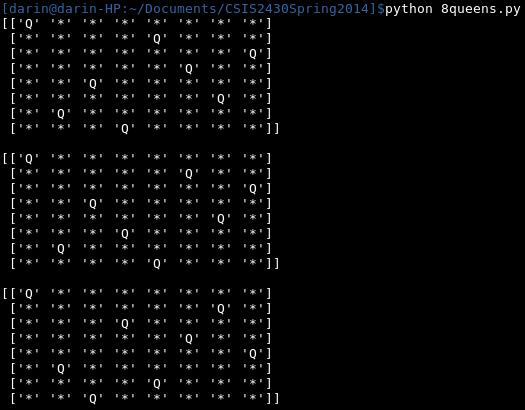
\includegraphics[width=470pt]{8_queens}

Screenshot of the first 3 solutions
\end{document}
